\documentclass[a4paper, 12pt]{article}
\usepackage{fullpage}
\usepackage{wrapfig}
\usepackage{float}
\usepackage{graphicx}
\usepackage{cite}
\usepackage{hyperref}
\usepackage{enumerate}
\usepackage{amsmath}
\usepackage{amssymb}
\author{Ryan J. Kinnear - 200273748 \\ Raza Rauf - 200300599}
\title{ENEL 417 - FPGA Based Software Defined Radio Peripheral}
\date{\today}

\begin{document}
\maketitle

\section{Background}
A software defined radio (SDR) is essentially a digital radio.  An analog front end device such as a DVB-T USB Dongle \cite{usb_dongle}, HackRF \cite{hackrf}, or the USRP \cite{usrp} receives and digitizes a radio frequency signal and sends the samples to a computer.  The ideal software defined radio consists of an analog to digital converter with one end connected directly to an antenna, and the other end connected to a computer.  A realistic implementation requires a significant analog component to digitize RF signals, as well as significant preprocessing on the digital signal (usually accomplished by an FPGA).

A complete SDR consists of an analog digitizing front end, and a large software system.  The point of this architecture is to achieve flexibility.  If the demodulator (ie. FM demodulator, QAM demodulator, PSK demodulator ...) is implemented in hardware as in a traditional radio, the receiver is only capable of extracting information (bits, or an base band analog waveform) from a certain type of signal.  For example, an FM radio receiver can't receive a 64QAM signal.  If the demodulator is implemented in software, the effort required to redesign to demodulate a new type of signal is reduced substantially.  Examples of SDR software are GNURadio \cite{gnu_radio} or SDR\# \cite{sdr_sharp}.  A software package needs to be integrated with a compatible RF front end.

The scope of our ENEL400/ENEL417 project is to implement the hardware front end, and a simple processing algorithm in an FPGA to demodulate broadcast FM radio.  Alternatively, or in addition, the system will be capable of sending samples to a computer to be demodulated in software.  There are no plans to integrate our hardware with either a full software radio suite, or any of our own real time processing code.  Although we may be able to write a (non real-time) demodulator that acts on a plain text file.

\section{System Specifications}
\begin{enumerate}
\item{The RF front end should be capable of receiving and converting an RF signal from between 50MHz and 340MHz into an IF frequency signal at 36.125MHz.  The bandwidth of this IF signal should be at least 6MHz.  Successful completion of this spec can be verified through a connection to a spectrum analyzer. \footnote{Note that some of our specifications are simply the specifications of the chip we are using.  We believe this is justified because getting the device to work requires a substantial design effort.  It is not as simple as just putting the chip on a breadboard and obtaining the expected performance.  Achieving the specifications of the device is not a straightforward task.}}
\item{The IF signal should be successfully digitized by an ADC, and send samples to an FPGA.  This spec can be verified through use of a signal generator and an oscilloscope.}
\item{The algorithm implemented in the FPGA should be able to demodulate a broadcast FM signal, and send the demodulated signal to a computer.  For example, demodulate CBC Radio 2 @ 96.9MHz.  This can be verified by sending test data generated by a script to the FPGA, running the algorithm on that, and then reading the processed data back to the computer.}
\item{The overall quality and noise levels of the system should be such that ``most'' people would consider the music quality to be ``reasonably acceptable''.  This is similar to the specifications for audio and video compression where a random sample of people must consistently rate the quality of the compression (subjectively) ``good''. For example, if 14/16 ENEL417 students rated the quality of the audio we receive as 7/10 or better, we have a very successful system.  This specification can be tested through a survey.  This specification assumes the previous 3 specifications are met.}
\end{enumerate}

\section{Work Load Plan}
The work load plan for our project is straightforward.  Ryan is designing and implementing the RF front end.  Raza is implementing everything in the FPGA, including the FM demodulation scheme, ADC controller, FMC interface, and system to send samples to a computer.  Any additional requirements, such as computer code will be scheduled as it arises.  The demarcation point between Ryan and Raza's work is the FMC connector on the SP601 FPGA development board.

\section{RF Front End Design (Ryan)}

\begin{figure}
\caption{System Diagram}
\label{fig:system_diagram}
\centerline{\includegraphics[width=15cm]{system_diagram.jpg}}
\end{figure}

Figure \ref{fig:system_diagram} is the design for the RF front end.  The FPGA element will be presented in the next section.  The items in the system diagram are numbered in orange to help the reader follow what is being referred to.

An antenna (1) is fed into a MAX3543 (6) television tuner/receiver.  This chip handles the main RF processing.  It filters out a roughly 8MHz band (primarily through the IF filter (7) which will be either a SAW filter or a LC ladder), anywhere between roughly 60MHz to 800MHz.  See figure \ref{fig:transfer_function}.  This is then downconverted to an apparently standard centre frequency of 36MHz.  The output is an analog differential signal.  This differential signal is fed into a fully differential operational amplifier (an ADC driver), and into the analog to digital converter.  The ADC is controlled by the FPGA.  Digital data is shifted 12 parallel bits at a time to the FPGA through an FPGA Mezzanine card (FMC \cite{fmc}).  This connector is conveniently present on the FPGA boards provided in the lab.

\begin{wrapfigure}{L}{0.5\textwidth}
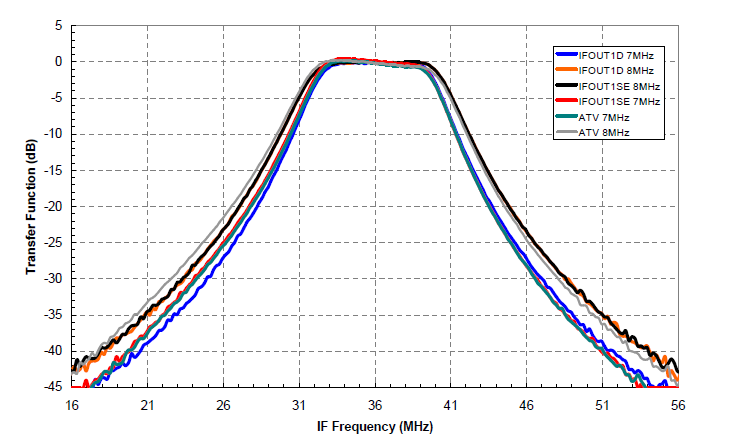
\includegraphics[width=.48\textwidth]{../../../transfer_function.png}
\caption{MAX3543 Transfer Function}
\label{fig:transfer_function}
\end{wrapfigure}

The MAX chip requires an I$^2$C interface to control various parameters such as the gain and the centre frequency of the RF filter.  This will be controlled by either the STM32 microcontroller, or a beaglebone black.  This is probably far easier than using the FPGA for control.

Finally, a digital stream of data will be shifted out of the FPGA into a plain text file on a computer.  The audio in this text file will be played with software on the computer.  Conveniently, the FPGA board has a UART to USB converter that can be used for this purpose.

\section{FPGA (Raza)}
FPGA’s are usually only used to down convert the incoming signal to a lower sampling rate that is then pushed to be processed on the computer. But we decided to do the processing right on the FPGA and then down convert the signal and send to the computer. After looking at many FM demodulation schemes, we decided on using the quadrature scheme due its good noise immunity and simplicity. First, the incoming signal is multiplied by cosine and sine to get the in-phase and quadrature components, respectively. Then, both the in-phase and quadrature are low pass filtered to attain the base band FM modulated signal. Then both signals are differentiated. The in-phase signal is multiplied by the differentiated quadrature and quadrature signal is multiplied by the differentiated in-phase. Both multiplications are summed together and scaled down. Now the FM signal is effectively demodulated. Because the sample rate is very high, 29 MSPS, we will need to down convert by a scale of 100. This new signal is then sent to the computer via UART. Ideally, a playable MP3 file is created on the computer and sent to the Echo Nest server to be identified and/or played on the computer.  The scheme can be seen graphically in figure \ref{fig:fpga}

Mathematically, the demodulation scheme can be described as follows:

\begin{equation}
  \phi_{FM}(t) = Acos\big(\omega_ct + k_f\int_{-\infty}^{t}m(t)dt\big)
\end{equation}

After I/Q sampling, we arrive at

\begin{equation}
\begin{aligned}
  &I(t) = Acos\big(\psi(t)) \\
  &Q(t) = Asin\big(\psi(t)) \\
  &\psi(t) = k_f\int_{-\infty}^{t}m(t)dt \\
\end{aligned}
\end{equation}

Thus to get back the message signal $m(t)$,

\begin{equation}
m(t) = \dot{\psi(t)} = \frac{d}{dt}\tan^{-1}{\Big(\frac{Q(t)}{I(t)}\Big)} =\
\frac{\dot{Q(t)}I(t) + \dot{I(t)}Q(t)}{I^2(t) + Q^2(t)}
\end{equation}

\begin{figure}
\centering
\includegraphics[width=.8\textwidth]{FPGA.jpg}
\caption{FPGA Demodulation Scheme}
\label{fig:fpga}
\end{figure}

As of now, we are strictly focusing on the heart of the project, which is RF front end, FMC input to the FPGA and then demodulation on the FPGA. Later, depending on time constraints, we will narrow down our specifications for for the later stages of the project. 
\section{Additional Concerns}

\begin{wrapfigure}{R}{0.5\textwidth}
\includegraphics[width=.48\textwidth]{QFN40.jpg}
\caption{MAX3543}
\label{fig:qfn40}
\end{wrapfigure}

\underline{Soldering} is a concern.  The MAX3543 (see figure \ref{fig:qfn40}) and the FMC connector will both be difficult to solder.  The MAX3543 is a 6x6mm 40pin QFN chip, I really did not appreciate how small this actually was until I saw it in person.  I have seen a number of YouTube videos of people soldering these and it does not seem like it is beyond our capability.  Tin the pads, use a heat gun, a lot of flux, and the chip falls into place.  The FMC connector will also pose a problem.  Dr. Zhang has said this is really the best connector for us.  I have read that using solder paste and a toaster oven or hotplate should work for this connector.

\underline{Gain Control}.  The MAX3543 should output a constant amplitude signal from it's differential output, however there is still a pin for IF gain.  It is stated in the data sheet that ``The MAX3543 is designed to control it's own RF gain ...'' however it is unclear how much AGC is provided by the MAX chip itself.  It may be necessary to control the gain ourselves.

\clearpage
\bibliography{../refs/fourth_year.bib}
\bibliographystyle{plain}
\end{document}
